% -*- latex -*-
%-----------------------------------------------------------------------
%;  Copyright (C) 2013
%;  Associated Universities, Inc. Washington DC, USA.
%;
%;  This program is free software; you can redistribute it and/or
%;  modify it under the terms of the GNU General Public License as
%;  published by the Free Software Foundation; either version 2 of
%;  the License, or (at your option) any later version.
%;
%;  This program is distributed in the hope that it will be useful,
%;  but WITHOUT ANY WARRANTY; without even the implied warranty of
%;  MERCHANTABILITY or FITNESS FOR A PARTICULAR PURPOSE.  See the
%;  GNU General Public License for more details.
%;
%;  You should have received a copy of the GNU General Public
%;  License along with this program; if not, write to the Free
%;  Software Foundation, Inc., 675 Massachusetts Ave, Cambridge,
%;  MA 02139, USA.
%;
%;  Correspondence concerning AIPS should be addressed as follows:
%;          Internet email: aipsmail@nrao.edu.
%;          Postal address: AIPS Project Office
%;                          National Radio Astronomy Observatory
%;                          520 Edgemont Road
%;                          Charlottesville, VA 22903-2475 USA
%-----------------------------------------------------------------------
%Body of final AIPSletter for 31 December 2013

\documentclass[twoside]{article}
\usepackage{graphics}

\newcommand{\AIPRELEASE}{December 31, 2013}
\newcommand{\AIPVOLUME}{Volume XXXIII}
\newcommand{\AIPNUMBER}{Number 2}
\newcommand{\RELEASENAME}{{\tt 31DEC13}}
\newcommand{\OLDNAME}{{\tt 31DEC12}}
\newcommand{\NEWNAME}{{\tt 31DEC14}}

%macros and title page format for the \AIPS\ letter.
\input LET98.MAC

\newcommand{\MYSpace}{-11pt}

\normalstyle

\section{General developments in \AIPS}

\subsection{Reduction of EVLA and ALMA data in \AIPS}

This \Aipsletter\ and those beginning in 2010 documents numerous
improvements to \AIPS\ that enable full calibration of Jansky VLA data
and most imaging operations as well.  The one exception is the
wide-band (bandwidth synthesis) deconvolution algorithm (``MSMFS'')
being developed in \CASA\ by Urvashi Rao Venkata, for which there is
no comparable function in \AIPS\@.  Calibrated $uv$ data may be
exported from \AIPS\ in ``UVFITS'' format for use in that program.
ALMA data may also be reduced in \AIPS, although the package is not
fully qualified to calibrate data from linearly-polarized feeds.  See
Appendix E of the \AIPS\ Cookbook, available via the \AIPS\ web site,
for details.

\subsection{\Aipsletter\ publication}

We have discontinued paper copies of the \Aipsletter\ other than for
libraries and NRAO staff.  The \Aipsletter\ will be available in
PostScript and pdf forms as always from the web site listed above and
will be shipped with all distributions of \AIPS\@.  It will be
announced on the bananas and mnj list servers and, usually, in the
NRAO e-News mailing.

\subsection{Current and future releases}

We have formal \AIPS\ releases on an annual basis.  We recommend a
full binary installation method for both the frozen and development
versions for MacIntosh OS/X (PPC and Intel chips), Solaris, and Linux
(32- and 64-bit) systems, but all architectures can do a full
installation from the source files.  If you develop \AIPS\ code
locally {\it or have system managers that forbid the use of\/} {\tt
  rsync} or {\tt cvs}, you will need to do a source-level
installation.  The current release is called \RELEASENAME\ and is now
``frozen.''  If you took a development copy of this version at some
earlier date, you should use the ``Midnight Job'' (MNJ) to bring it up
to date.  You need to run a MNJ only once in 2013 to convert your copy
of \RELEASENAME\ into the frozen version.  However, when patches to
\RELEASENAME\ are announced, you may apply them with the MNJ\@.  This
\Aipsletter\ is intended to advise you of corrections and improvements
in this release.

We have begun a new version, called \NEWNAME, which is now under
development by the \AIPS\ Group.  You may fetch and install a complete
copy of this version at any time.  Having fetched \NEWNAME, you may
update your installation whenever you want by running the MNJ\@.  This
uses {\tt cvs}, {\tt rsync}, and/or transaction files to copy all
changed text files and then to copy the binary files or to compile the
code selectively based on the code changes and compilations we have
done.  We expect users to take their source-only or binary version of
\NEWNAME\ \AIPS\ over the Internet (via \emph{anonymous} ftp).  Both
versions require you to copy the installation procedure {\tt
  install.pl} via {\tt ftp}; the source-only version also requires you
to ftp the 115-Mbyte {\tt   \NEWNAME.tar.gz} compressed tar file.
Linux sites will almost certainly have {\tt cvs} installed; other
sites may have installed it along with other GNU tools.  Secondary
MNJs will still be possible using {\tt ssh} or {\tt rcp} or NFS as
with previous releases.  We have found that {\tt cvs} works very well,
although it has one quirk. If a site modifies a file locally but in an
\AIPS-standard directory, {\tt cvs} will detect the modification and
attempt to reconcile the local version with the NRAO-supplied version.
This usually produces a file that will not compile or run as intended.
Use a new name for the task or put a copy of the task and its help
file in a private disk area instead.

\AIPS\ is now copyright \copyright\ 1995 through 2013 by Associated
Universities, Inc., NRAO's parent corporation, but may be made freely
available under the terms of the Free Software Foundation's General
Public License (GPL)\@.  This means that User Agreements are no longer
required, that \AIPS\ may be obtained via anonymous ftp without
contacting NRAO, and that the software may be redistributed (and/or
modified), under certain conditions.  The full text of the GPL can be
found in the \texttt{15JUL95} \Aipsletter\ and is included with every
distribution in file {\tt \$AIPS\_ROOT/{\it release-name}/COPYING}\@.


\subsection{Installing a new version}

If compiling locally, new releases must be installed from the tar ball
for that release.  If using the binary installation, a full new
installation must also be done with {\tt rsync}.  The {\tt cvs} system
used in the MNJ requires this.  When installing a new \AIPS\ release
in a system that already has a previous release, we recommend that
{\tt install.pl} be used and that the previous release be left in
place, at least until the new installation has been verified.  If you
do this, then you will not have to re-edit the disk, printer, and tape
lists and can simply skip all those pages in the {\tt install.pl}
menus.  The old {\tt \$HOME/.AIPSRC} file may be left in place, but it
will need to be edited.  The lines giving the {\tt DOWNLOADED} and
{\tt UNPACKED} parameters should be cleared and the {\tt CCOMOPT} line
should be changed to point to the current release rather than the
previous one.  If you have made a special version of {\tt
  do\_daily.{\it host}}, you should preserve it under a new name and
restore it after the install.  If you have an odd set of \AIPS\
versions, the {\tt \$AIPS\_ROOT/AIPSPATH.*SH} files may need to be
edited after the install to set the desired versions.

{\tt 31DEC09} contains a change in the format of antenna files.
Previous releases will not understand the antenna coordinates for
arrays that were traditionally left-handed (VLBI primarily).  The
format change occurs automatically when any {\tt 31DEC09} or later
antenna-file specific code reads the file, after which older releases
will have difficulties.  Note that the only version which we patch for
major errors is \RELEASENAME; even \OLDNAME\ is no longer changed.

\section{Preview of coming attractions}

The \NEWNAME\ release already contains a few changes that we decided
were a bit risky or not needed in \RELEASENAME\@.  {\tt APCAL} will
now loop over subarray.  The format of the {\tt TGET}/{\tt TPUT} file
was changed to incorporate the names, sizes, and types of the adverbs
present in the file.  Subsequent {\tt TGET}s will change the values of
these adverbs and report any differences between the {\tt TGET} file
and the current {\tt INPUTS} file.  This will prevent adverb values
from being messed up by a {\tt TGET} when there are new adverbs in the
{\tt INPUTS} file.  {\tt RLDLY} has the option to average solutions
over all possible reference antennas rather than depending on just
one.  A new appendix to the \Cookbook\ has been completed.  It is a
simplified guide to EVLA P-band data reduction in \AIPS\@.  The EVLA
and VLBA data reduction pipeline procedures have been brought up to
date.  After some more testing, they will be released in {\tt
  31DEC14}\@.  {\tt BLSUM} will soon have the ability to make real
plot files in addition to, or instead of, its printer plots.

\vfill\eject

\section{Improvements of interest to users in \RELEASENAME}

We expect to continue publishing the \Aipsletter\ every six months
along with the annual releases.  There are several new tasks released
in the last six months.  New tasks in the last six months include
{\tt BPWGT} to use the bandpass table to estimate channel-dependent
weights, {\tt HA2TI} to convert data sets with hour angle as the
``time'' into true times, {\tt SNP2D} to convert a single-channel
phase calibration into a delay suitable for wide bandwidths, {\tt
  ALVAR} to estimate the Allen variance of visibility phases, {\tt
  REIFS} to convert a data set into multiple IFs allowing the new IFs
to include data from more than one input IF, {\tt BDAPL} to apply a
{\tt BD} table found by {\tt BLCHN} to another data set, {\tt ZEMAN}
to fit Zeeman splitting models to image cubes with interactivity, and
{\tt SPMOD} to add spectral-line models to a $uv$-data set.  See below
for more details.

In the first six months of \RELEASENAME\ the new tasks were {\tt
RMFIT} to fit polarization models to Q/U cubes interactively, {\tt
DSKEW} to remove coordinate skew from input (usually optical) images,
{\tt FTFLG} to edit {\it uv} data interactively in a frequency-time
display with all baselines averaged, {\tt CLVLB} to apply calibration
to correct VLBI data for phase-stopping positions away from the
pointing position, {\tt VLAMP} to determine system temperature
calibration for the phased VLA in VLBI observations, and {\tt PCVEL}
to include planetary velocities when correcting {\it uv} data spectra
to be centered on a line at the source.  The interactive
Gaussian-fitting task {\tt XGAUS} was overhauled to become a much more
usable tool to fit large spectral cubes.  The handling of more global
coordinate types was expanded and brought up to more modern standards
to handle images, primarily optical, now being brought into \AIPS\@.
A fifth name group ({\tt IN5NAME}, {\it et al.}) was added with new
verbs {\tt GET5NAME}, {\tt M5CAT}, {\tt U5CAT}, {\tt IM5HEAD}, and
{\tt Q5HEADER} to support it.

Normally, bugs which appear in an \AIPS\ {\tt TST} version and then
are fixed in that same version before its release get little or no
discussion in the \Aipsletter\@.  Since a rather large number of sites
now install the {\tt TST} version of \AIPS\ during its development,
this is somewhat of an oversight.  We urge you to run the ``Midnight
Job'' at least once after \RELEASENAME\ is frozen to bring it up to
date and to fix all bugs of this sort.  We urge active sites to use
the MNJ and, when something odd occurs, to examine {\tt CHANGE.DOC}
using the cgi tool available from the \AIPS\ documentation web page
({\tt http://www.aips.nrao.edu/aipsdoc.html}).  Please do not hesitate
to e-mail {\tt daip@nrao.edu} with any questions or suspicions that
there are problems.

\subsection{UV data}

\subsubsection{Primary calibration source spectra}

Task {\tt SETJY} is provided with the best possible fluxes and
spectral shapes available.  These parameters are provided by Rick
Perley and Bryan Butler.  In 2013, {\tt SETJY} was given
time-dependent fluxes for 3C48, 3C138, and 3C147, low frequency fluxes
from Anna Scaife and George Heald, and spectra for the stable sources
3C123, 3C196, and 3C295\@.  {\tt SETJY} was also given a new option
{\tt VANT} to compute the velocity of each source at its first scan,
like {\tt VCAL} but with respect to a specified antenna rather than
the center of the Earth.  Bugs affecting the velocity computation were
fixed.

Tasks {\tt BPASS} and {\tt CPASS} need to know source spectral index
in order to correct the bandpass functions to a spectral index of
zero.  Both tasks were given knowledge of all spectral energy
distributions known to {\tt SETJY}\@.  {\tt BPASS} was corrected to
allow separate spectral indexes for each calibration source and to fit
the fluxes in the {\tt SU} table for any calibration source not in the
list of known sources.  {\tt BPASS} was also corrected for an error in
separating closely-spaced scans.

\begin{description}
\myitem{BPWGT} is a new task to set the weights of data based on the
               values in the bandpass table.  Various functions of the
               bandpass values are allowed.
\myitem{HA2TI} is a new task to convert hour angles back to legitimate
               times in a data set which had been through {\tt
               TI2HA}\@.  This allows data from multiple days to be
               run through {\tt STUFFR} and then converted back for
               use by tasks that require real times (such as {\tt
               UVFIX}, {\tt CASA})\@.
\myitem{SNP2D} is a new task to convert the phase calibration found in
               one IF at one channel (\eg\ at a maser line at the
               phase center) into a delay suitable for application to
               a wide bandwidth.
\myitem{SPLIT} and {\tt SPLAT} ran into trouble when a source was
               found to have no data.  The error messages have been
               improved and history card counters reset.  {\tt SPLAT}
               copies only those flag tables with a version greater
               than the one being applied (when making a multi-source
               output file.)
\myitem{UVFND} now offers the {\tt NCHAV} option so that tests are
               performed on a channel average rather than a noisier
               single-channel value.
\myitem{LISTR} can now list ${\rm P}_{\rm sum}$ and  ${\rm P}_{\rm
               dif}$ from {\tt SY} tables with {\tt OPTYPE 'GAIN'}\@.
\myitem{ALVAR} is a new task to compute the Allen variance of complex
               visibilities in several ways.  It prints the answers as
               a function of baseline and IF which may be used to
               evaluate the performance of the telescope.
\myitem{TYAPL} was changed to give ``skipped'' antennas (due to bad
               values in the {\tt SY} table and the {\tt CUTOFF}
               adverb) values equal to the average of those antennas
               which were not skipped.  While not perfect, this will
               put the data weights on a similar basis.
\myitem{RFLAG} was given two more options to flag whole baselines in
               any spectral window that has fluxes exceeding the new
               parameters ({\tt FPARM(15)} and {\tt FPARM(16)})\@.
\myitem{REIFS} is a new task to divide a data set into multiple IFs.
               The new IFs can include data from more than one input
               IF which allows the task to retain IF-dependent values
               from the input tables.
\myitem{SPFLG} was given double-precision counters to avoid overflows,
               was changed to handle missing sources in the source
               table, and was fixed to label sub-images correctly.
               {\tt DPARM(4) = 2} is a new option to divide not only
               by the source flux (as a function of IF) but also to
               determine a spectral index and use it to determine the
               flux to be divided into each channel.
\myitem{UVPLT} was given the {\tt DOSCALE} option to divide the
               plotted fluxes by those in the source table, including
               optionally a spectral index also found from the source
               table values.  Thus the plot is of normalized flux.
\myitem{CLIP}  was given the {\tt DOSCALE} option to divide the tested
               fluxes by those in the source table, including
               optionally a spectral index also found from the source
               table values.  Thus the clipping is based on normalized
               flux and so might apply to multiple sources.
\myitem{BLCHN} was changed to correct the answers for the calibration
               source spectral index.  The ``known'' sources have
               spectral indexes available, unknown sources will find
               the spectral index from the source table, or the user
               may specify a spectral index (and curvature).  The
               correction may be turned off if desired.
\myitem{BDAPL} is a new task to apply a {\tt BD} table found by {\tt
               BLCHN} to another data set (\ie\ not the one input to
               {\tt BLCHN}\@.
\myitem{USUBA} was changed to write subarray value 0 into those tables
               for which the new subarray values are not readily
               determined.  Only tables with subarray, source, time,
               {\it and} antenna columns will get the newly determined
               subarray numbers.  All tasks should understand that
               subarray 0 means all subarrays.
\end{description}

\subsection{Imaging}

\begin{description}
\myitem{SUBIM} was given a {\tt ZINC} option to allow selecting every
               $n^{\rm th}$ plane.  The option to determine the
               average, minimum, or maximum over the ${\tt XINC}
               \times {\tt YINC} \times {\tt ZINC}$ voxel was
               retained.  Errors in the old implementation of this
               option were corrected.
\myitem{TRANS} messed things up badly when swapping rows with a row
               reversal.  The task usually died from writing off the
               end of the file.  The matter has been fixed.
\myitem{IMAGR} was corrected to compute the average included frequency
               correctly.  Previously it assumed that the frequencies
               were in a monotonic and regular sequence.
\myitem{TVMOVIE} can be replicated in an animated gif for use in
               talks.  Information about how to do this was added to
               the help file.
\end{description}

\subsection{Analysis}

\subsubsection{Interactive analysis of spectral cubes}

The previous \Aipsletter\ reported on the overhaul of {\tt XGAUS} to
make a truly useful, interactive task to fit Gaussians to
spectral-line cubes.  It also reported the creation of a task to fit
rotation measures to cubes of Stokes Q and U\@.  Tests of {\tt RMFIT}
show that it correctly resolves RM components which are totally
blended in Faraday rotation measure synthesis methods.  These tasks
received considerable effort over the last six months as well.  The
most notable changes are to allow {\tt XGAUS} to fit up to 8 Gaussians
at every pixel, to allow both tasks cubes up to 8192 pixels on the $x$
axis, and, optionally, to fit spectral index in {\tt RMFIT}\@.
Both tasks were changed to display the image step wedge more clearly
(including a line drawn around the image), to handle the setting of
blotch regions with more forgiveness for user error, to display and
manage images larger than the TV display, to display the fit results
and errors more completely, to try additional methods for finding the
next initial guess, to solve for the fit even when a parameter or
component is not fit, and to allow restarts on smaller regions
interior to the region used initially.  {\tt RMFIT} was changed to
function without a total-intensity input image, to allow the user to
set the Q and U display ranges, and to record more things in the {\tt
RM} table including the rms of the fit evaluated with and without
weighting.  {\tt XGAUS} was changed to drop a number of adverbs that
are no longer useful in the overhauled task.

A new task, based on {\tt XGAUS} has now been written.  It is called
{\tt ZEMAN} and solves at each spectrum the equation $ V(c) = A I(c) +
0.5 B dI(c)/dc$ where $V(c)$ is the Stokes V cube at channel $c$ and
$I(c)$ is the total intensity spectrum.  The task also offers the
option of using the {\tt XG} table produced by {\tt XGAUS} and solving
$V(c) = A I(c) + 0.5 \sum [ B_i dG_i(c)/dc ]$, where $G_i$ is the
$i$'th Gaussian component.  {\tt ZEMAN} has much of the same structure
as {\tt XGAUS} and {\tt RMFIT} although the fit is linear and not as
difficult as the Gaussian and rotation measure ones.  In the end, {\tt
ZEMAN} will produce images of $A$ and $B$ or $B_i$.  The Gaussian
model for {\tt ZEMAN} has been found correct answers in data of poor
spatial resolution (in which 2 lines overlap spatially) when compared
to the same region observed earlier with good spatial resolution.

\subsubsection{Other analysis}

\begin{description}
\myitem{SPMOD} is a new task that adds a model to an existing
               $uv$-data set.  The model is of spectral lines of
               specified spatial type, position, and extent and
               frequency position and Gaussian width.  Up to 9999
               components may be specified.
\myitem{SAD,} {\tt IMFIT}, and {\tt JMFIT} were corrected to return
               positive error bars even when the component peak flux
               is negative.
\myitem{SLFIT} was changed to scale with the slice minimum and maximum
               rather than those of the image as a whole.  Changed to
               use double precision to deal with extreme images.
\myitem{FARS} was corrected to use buffers large enough for the images
               in allowed.
\end{description}

\subsection{General and system matters}

\begin{description}
\myitem{RUN} files may now contain {\tt RUN} commands, up to a nesting
               level of 20.  The ``verb'' {\tt COMPRESS} uses {\tt
               RUN} and so counts as one of the 20.
\myitem{install.pl} was changed to drop the dependence on certain Perl
               ``packages'' which are not always available.
\myitem{Unix} sockets have predictable names which are used by \AIPS\
               but this now fails on Mac systems.  The start-up
               procedures were changed to skip the test on the display
               name on Macs.  This does interfere with the option to
               have one computer display on multiple computers, but
               Macs are not usually used in that way.
\myitem{Tables} may have flagged rows, since this option is directly
               available to the user.  All table routines should
               return flagged rows to the calling routine with a
               negative error code to indicate the flagging.  Numerous
               table routines that did other things were corrected.
               Calling routines should deal with flagged rows
               appropriately (skip them usually).
%\myitem{CookBook} was updated to match the changes over the last year.
%               A new chapter on P-band data reduction in \AIPS\ was
%               added.
\end{description}
\eject

\section{Patch Distribution for \OLDNAME}

Because of the extensive use of binary installations, we now patch the
master copy of the most recently frozen version.  Older versions are
not corrected even for egregious errors.  Thus, \OLDNAME\ was patched
during 2013 and \RELEASENAME\ will be patched as needed during 2014.
Your copy of them may be corrected simply by running a Midnight Job.
Information about patches and the code may be found using links from
the main \AIPS\ web page or by  {\it anonymous} \ftp\ to the NRAO
server {\tt ftp.aoc.nrao.edu}.  Documentation about patches to a
release is placed on this site at {\tt pub/software/aips/}{\it
  release-name} and the code is placed in suitable sub-directories
below this.  Patches to older releases are kept here as well, but they
will require local compilation.

The \OLDNAME\ release is no longer available for installation and will
no longer receive patches even for egregious errors.  It had a number
of important patches during 2012.  They are
\begin{enumerate}
  \item\ Bandpass calibration was not applied to enough channels to
         support frequency smoothing afterward. {\it 2013-01-16}
  \item\ Tick increments were computed with an erroneous round-off
         parameter leading some tick marks to be plotted at offset
         values. {\it 2013-01-29}
  \item\ {\tt POSSM} had a variety of irritating bugs. {\it
         2013-02-05}
  \item\ {\tt FITLD} turned off {\tt DIGICOR} corrections when the
         array name was not VLBA. {\it 2013-02-05}
  \item\ {\tt FITLD}, after correction 4, failed if it could not make
         a {\tt CQ} table. {\it 2013-02-18}
  \item\ {\tt CL2HF} aborted because of an internal name conflict. {\it
         2013-02-19}
  \item\ {\tt PRTAB} had a format issue with large F formats ({\tt
         NDIG} $\le 0$). {\it 2013-03-01}
  \item\ {\tt COMB} did not do {\tt POLC} correctly when using
         constant noise values.  {\it 2013-04-04}
  \item\ {\tt AFARS} had a header bug causing it to try to write too
         much.  {\it 2013-04-05}
  \item\ {\tt FITLD} could get the {\tt EQUINOX} wrong in the {\tt SU}
         table  with FITS-IDI input. {\it 2013-04-11}
  \item\ {\tt COMB} messed up scaling when combining two images with
         one of them not {\tt JY/BEAM}\@.  {\it 2013-05-03}
  \item\ {\tt FITLD} had a bad warning message, causing aborts on some
         machines.  {\it 2013-05-21}
  \item\ {\tt BPASS} rounded times outward for each scan by too much.
         {\it 2013-06-17}
  \item\ {\tt SETJY} used Perley 2010 coefficients but reported Perley
         2013 coefficients.  {\it 2013-06-26}
    \item\ {\tt IMAGR} computed the actual average frequency wrongly.
         {\it 2013-07-03}
    \item\ {\tt IMFIT} and {\tt JMFIT} could return negative error
         bars when the object was negative. {\it 2013-07-07}
    \item\ {\tt TRANS} messed up when reversing the order of an axis
         it was also swapping. {\it 2013-07-17}
    \item\ {\tt PRTAB} had formatting issues with large tables with
         many blanked values. {\it 2013-07-25}
    \item\ {\tt SU} table access was incorrect in some routines
         including widely used ones.  {\it 2013-07-29}
    \item\ {\tt SPFLG} had a gridding counter which could overflow
         with modern data sets. {\it 2013-08-16}
    \item\ {\tt PRTAB} had formatting issues with required E formats
         in F-format modes. {\it 2013-08-23}
    \item\ {\tt SETJY} and {\tt CVEL} were affected by a bad variable
         in setting the Doppler velocity and the former omitted the
         system velocity when setting source velocities. {\it
           2013-10-21}
    \item\ {\tt ISPEC} on an image with an {\tt FQID} axis could fail.
         {\it 2013-10-24}
\end{enumerate}

\vfill\eject

\section{\AIPS\ Distribution}

From the NRAO system logs, we count apparent MNJ accesses, downloads
of the tar balls, and {\tt rsync} accesses by unique IP address.
Since DSL and some university and other connections may be assigned
different IP addresses at different times, this will be a bit of an
over-estimate of actual sites.  However, a single IP address is often
used to provide \AIPS\ to a number of computers, so these numbers are
at the same time an under-estimate of the number of computers running
current versions of \AIPS\@.  In 2013, a total of 307 different IP
addresses downloaded the frozen form of \OLDNAME\ and 1013 IP
addresses downloaded \RELEASENAME\ in tarball or binary form.  Fully
1264 IP addresses accessed the NRAO cvs master.  Each of these has at
least installed some version of \AIPS\ and 365 appear to have run the
MNJ at least occasionally.  The total number of unique IP addresses in
these three lists was 1937.  The table below shows these numbers as a
function of year since we began recording them.  The attached figure
shows the cumulative number of unique sites, cvs access sites, and
download sites known to us as a function of week in 2013.  The numbers
for 2012 are also plotted and show an increase in 2013 in all numbers
except those for {\tt cvs}, perhaps due in part to a VLBI workshop
which used \AIPS\@.

\vfill
\begin{center}
\begin{tabular}{|rrrrrrrrr|}
\hline
%year & {\tt TST} name & {\tt NEW} name & \hspace{1em}{\tt TST} &
% \hspace{1em}{\tt NEW} & {\tt TST binary} & {\tt NEW} binary &
% \hspace{1em}{\tt cvs} & Total unique \\
 & & & & & {\tt TST} & {\tt NEW} & & Total \\
\noalign{\vspace{-1mm}}
year & {\tt TST} name & {\tt NEW} name & \hspace{1em}{\tt TST} &
 \hspace{1em}{\tt NEW} & binary & binary &
 \hspace{1em}{\tt cvs} & unique \\
\hline
2004 & {\tt 31DEC04} & {\tt 31DEC03} &  808 & 196 &      &     &  797
 & 1276 \\
2005 & {\tt 31DEC05} & {\tt 31DEC04} &  832 & 246 &  299 &  48 &  982
 & 1460 \\
2006 & {\tt 31DEC06} & {\tt 31DEC05} &  806 & 191 &  402 &  94 & 1050
 & 1398 \\
2007 & {\tt 31DEC07} & {\tt 31DEC06} &  965 & 277 &  669 & 161 & 1385
 & 1811 \\
2008 & {\tt 31DEC08} & {\tt 31DEC07} & 1058 & 246 &  986 & 303 & 1667
 & 2107 \\
2009 & {\tt 31DEC09} & {\tt 31DEC08} & 1228 & 307 & 1082 & 478 & 1855
 & 2399 \\
2010 & {\tt 31DEC10} & {\tt 31DEC09} & 1228 & 307 & 1203 & 477 & 1914
 & 2416 \\
2011 & {\tt 31DEC11} & {\tt 31DEC10} & 1105 & 270 & 1064 & 424 & 1747
 & 2228 \\
2012 & {\tt 31DEC12} & {\tt 31DEC11} &  940 & 284 & 1028 & 396 & 1309
 & 1698 \\
2013 & {\tt 31DEC13} & {\tt 31DEC12} & 1014 & 307 &  990 & 443 & 1264
 & 1937 \\
\hline
\end{tabular}
\end{center}
\vfill
\centerline{\resizebox{!}{4.6in}{\includegraphics{FIG/PLOTIT13b.PS}}}
\eject

% Order form and mailer page
%\cleardoublepage
\pagestyle{empty}
%\vfill
%\centerline{\resizebox{!}{23.3cm}{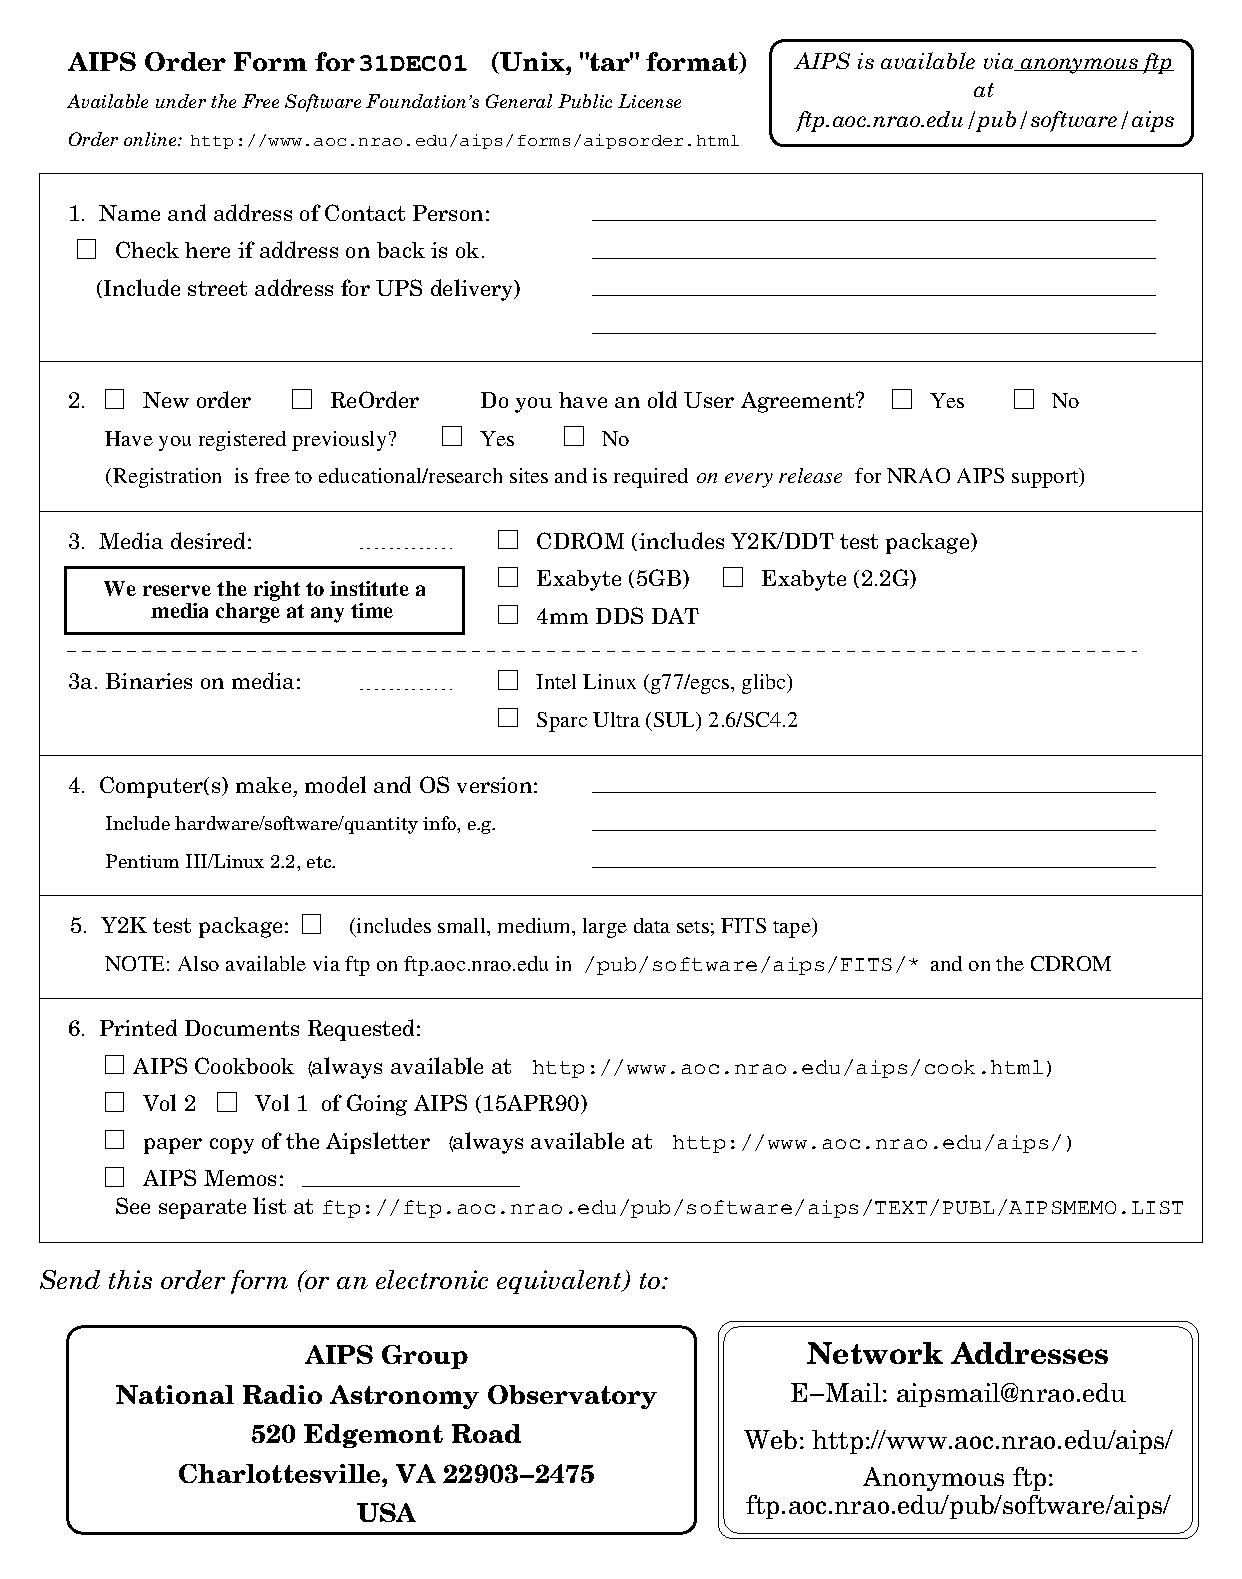
\includegraphics{FIG/AIPSORDER.PS}}}
%\vfill\eject
\vbox to 4.4in{
\vspace{12pt}
%\centerline{\rotatebox{-90}{\resizebox{!}{3.5in}{%
%\includegraphics{FIG/Mandrill.color.plt}}}}
\centerline{\resizebox{!}{3.5in}{\includegraphics{FIG/Mandrill.eps}}}
\vspace{12pt}
\centerline{{\huge \tt \AIPRELEASE}}
\vspace{12pt}
\vfill}
\phantom{...}
\centerline{\resizebox{!}{!}{\includegraphics{FIG/AIPSLETS.PS}}}

\end{document}
